\documentclass[12pt]{article}%[12pt, twocolumn]{aastex631}

\usepackage{graphicx}
\usepackage{float}
\usepackage{amsmath}
\usepackage{natbib}
\usepackage{url}
\usepackage{subcaption}

\usepackage{afterpage}

\usepackage{xcolor}
\usepackage{listings}

\lstdefinelanguage{SQL}{
    keywords={SELECT, FROM, WHERE, AND, OR, AS, JOIN, LEFT, RIGHT, INNER, OUTER,
              ON, GROUP, BY, ORDER, DESC, ASC, LIMIT, CASE, WHEN, THEN, ELSE,
              END, IS, NOT, NULL, COUNT, AVG, SUM, MIN, MAX, DISTINCT},
    keywordstyle=\color{blue}\bfseries,
    comment=[l]{--},
    commentstyle=\color{gray}\itshape,
    stringstyle=\color{red},
    morestring=[b]',
}

\lstset{
    basicstyle=\ttfamily\small,
    breaklines=true,
    frame=single,
    columns=fullflexible,
    keepspaces=true,
    showstringspaces=false,
    captionpos=b
}

\bibliographystyle{plainnat}

\usepackage[colorlinks=true,
            linkcolor=blue,
            citecolor=blue,
            urlcolor=blue]{hyperref}

\title{\textbf{Transit Exoplanet Surveys and False Positive Challenges}}

\date{April 6th 2026}
\author{\textbf{Author}: Aaryan Thusoo \\ \textbf{Supervisor}: Prof. Vincent Van Eylen}

\begin{document}

\maketitle

\newpage{}
\begin{abstract}
    The use of convolutional neural networks (CNN) to analyse patterns in transiting exoplanets has been observed as an upcoming method in filtering false positive signals. However, for best results, papers focus on preprocessing and cleaning the data heavily to make classification easier on the model. This paper focuses on improving the model to handle Kepler raw data for classification. Using lightly processed data, a binary and multiclass CNN were developed to classify light curves from Kepler as transit or shallow/deep eclipsing binaries. The binary model showed impressive results with \textbf{(How much)}\% accuracy score while the multiclass model had an accuracy of \textbf{(What score?)}\%. The main distinction comes from the tricky nature of shallow eclipsing binaries which are very common in observation. This research focuses on the developing process of using machine learning models to search for exoplanets with minimal manual processing requirements.
\end{abstract}

\section{Introduction}

Prior to 1992, the existence of planets beyond the Solar System was largely speculative. This changed with the first observational evidence of extrasolar objects in the early 1990s \citep{First_Exoplanet, First_Exoplanet_RV}. These confirmations transformed the field from theoretical speculation into an observational science. Since then, the rate of discovery has increased rapidly, and by 2008 over 263 exoplanet systems had been confirmed \citep{Exoplanet_numbers_2008}. As of August 2026, over 6000 exoplanets have been confirmed, and thousands more are candidates awaiting further observation \citep{christiansen2025nasaexoplanetarchiveexoplanet}.\footnote{Confirmed planet counts obtained from the NASA Exoplanet Archive Confirmed Planets Table, accessed March 2026: \url{https://exoplanetarchive.ipac.caltech.edu/}}

This rapid growth in detections has been driven by advances in observational techniques and instrumentation. 51 Pegasi b was the first exoplanet discovered orbiting a Sun-like star. It was detected using radial velocity (RV) measurements of its host star \citep{First_Exoplanet_RV}. As the number of candidates increased, manual and low-throughput detection approaches became inefficient. Although radial velocity measurements remain widely used, transit photometry has become the dominant detection method \citep{How_Many_Transits}.

When analysing transit data, a major source of false positive transit-like signals is eclipsing binary systems, where two stars orbit one another and periodically pass in front of each other from the observer's perspective \citep{2018ApJS..235...38T, Morton_2016}. These systems can produce repeated decreases in observed flux that resemble planetary transits, making them an important contaminant when identifying exoplanet candidates.

This paper trains machine learning models to classify light curves collected from NASA's \textit{Kepler} mission as either transiting exoplanets or eclipsing binaries. Since eclipsing binaries and other astrophysical systems can produce transit-like false positive signals, an automated classifier could reduce the need for manual vetting. Previous studies have explored machine learning approaches for false positive identification, often using heavily processed or phase-folded light curves. The goal of this work is to test whether a model can achieve useful classification performance using relatively limited preprocessing of the input data.


\section{Extrasolar Planets Detection} \label{sec:Extrasolar_Planets_Detection}

\subsection{Exoplanets} \label{sec:Exoplanets}

Figure~\ref{fig:exoplanet_methods_figure} shows the distribution of all confirmed exoplanets by discovery method, as obtained from the NASA Exoplanet Archive \citep{NASA_Exoplanet_Tool, Exoplanet_NASA_Table}. The figure illustrates that transit photometry (purple) is currently the most successful detection method, followed by radial velocity measurements (green), although many more methods have been developed to find new planets. The discovery method refers to the first technique used to determine the presence of an exoplanet. Once an initial detection is reported, the host system becomes the focus of further observations. To improve confidence in exoplanet candidates, astronomers tend to use multiple detection methods \citep{Confirm_w_multiple}.

\begin{figure}[h]
    \centering
    
\includegraphics[width=1.2\linewidth]{Images/exoplanet_method_numbers}
    \caption{The rate of exoplanet discoveries has increased dramatically since 1995\protect\footnotemark[2]. Transit photometry grew rapidly as technology improved becoming the most common detection method.}
    \label{fig:exoplanet_methods_figure}
\end{figure}

\footnotetext[2]{\url{https://ourworldindata.org/grapher/cumulative-exoplanets-by-method}}

\subsection{Light Curves} \label{sec:Lc_Detection}

Transit photometry observes the flux from stars searching for periodic decreases in brightness caused by a planet crossing the stellar disk \citep{Exoplanet_Detection_Methods}. This method has become the most successful in exoplanet detection, with over 4300 confirmed planets \citep{Num_Transit_Exoplanets_Discovered}. This success is due to its relatively simplistic process and easy parameter estimation directly from the light curve \citep{Transit_Method}. Figure~\ref{fig:WASP-104 Full} illustrates this pattern with a light curve of star WASP-104 highlighting the consistent dip in the observed flux \citep{2003ApJ...585.1038S}.

\begin{figure}[h]
    \centering
    
\includegraphics[width=0.75\linewidth]{Images/Lightcurves/WASP-104b_transit.jpg}
    \caption{Photometric light curve of the WASP-104 system showing repeated transit events of the exoplanet WASP-104 b. The horizontal axis is time in Barycentric Julian Date (BJD - 2450000), while the vertical axis shows the measured stellar flux. Each downward spike corresponds to a planetary transit, where the planet passes in front of its host star and blocks a small fraction of the starlight. The black curve shows the original observed light curve, while the red curve shows the processed or detrended data used to highlight the transit signal. Reproduced from \citep{WASP-104b_Lightcurves} (Figure 1).}
    \label{fig:WASP-104 Full}
\end{figure}


\begin{align}
    \delta F \approx \left(\frac{R_p}{R_*}\right)^2 \label{eq:flux_depth}
\end{align}

Astronomers analyze many features in transit light curves which describe key parameters of the exoplanet system. The depth of the transit provides a direct measurement of the planet-to-star radius ratio. This relation is depicted in Equation~\ref{eq:flux_depth} above. Here $\delta F$ is the change in normalized flux caused by the transit dip. $R_p$ and $R_*$ represent the radius of the exoplanet and its host star respectively.

\begin{figure}[H]
    \centering
    
\includegraphics[width=0.8\linewidth]{Images/Lightcurves/transit_anatomy.png}
    \caption{A breakdown of the parameters researchers look for in transit light curves. Transits are broken into four segments labelled $t_I$ to $t_{IV}$. $\tau$ is used to represent ingress and egress times which occur between $t_I$ and $t_{II}$ or $t_{III}$ and $t_{IV}$ respectively. $T$ is the elapsed time for which the full planet is transiting in front of its host star. These times are heavily affected by the impact parameter $b$. Reproduced from \citet{2010exop.book...55W} (Figure 2).}
    \label{fig:Transit_Anatomy}
\end{figure}

Stars also exhibit limb darkening, a phenomenon in which the stellar surface appears dimmer near the limb due to variations in temperature and optical depth within the stellar atmosphere. The curvature of the transit dip is influenced by stellar limb darkening. The initial and final phases of a transit are known as ingress and egress respectively \citep{2003ApJ...585.1038S}. The total transit duration, ingress/egress duration, and overall transit shape provide information about the impact parameter, orbital inclination, and stellar density \citep{2010exop.book...55W}. More detailed transit fitting can be used to constrain planetary and orbital properties more generally \citep{2023MNRAS.520.4103H, 2015ApJ...808..126V}. Figure~\ref{fig:Transit_Anatomy} illustrates the morphology of a typical transit light curve and the parameters encoded within it. The mathematical relationships between transit light-curve features and the physical properties of the system are summarized in Appendix~\ref{sec:Transit_Geometry}.
\subsection{Detection Challenges} \label{sec:Detection_Challenges}

Many factors, including stellar variability and instrumental noise, can affect the accuracy of light-curve analysis in transit photometry. These effects not only influence parameter estimation but can also lead to false-positive detections. A false positive occurs when a signal is incorrectly interpreted as a transit even though it was not caused by an exoplanet-star system. Several physical and instrumental effects can produce signals that mimic transit patterns \citep{Morton_2016}.

\subsubsection{Stellar Variability}

Stars exhibit time-variable activity across their surfaces. Sunspots reduce the local surface brightness while faculae lead to an increase in the surrounding region. The timescale and amplitude are dependent on factors such as effective temperature \citep{2012IAUS..285..364M}. When a transit passes over these active regions, this can cause small fluctuations in the transit profile \citep{2013A&A...556A..19O}. Active regions evolve and rotate across the stellar surface, introducing time-dependent variability. This rotational modulation can produce broad, quasi-periodic trends in the light curve that may obscure or imitate shallow transit signals. As a result, stellar variability can affect both the detection of transits and the estimation of planetary parameters derived from the light curve \citep{Bonomo_2009}.

\subsubsection{Instrumentation} 

Missions focused on transit observations must rely on precise differential photometry. The \textit{Kepler} mission \citep{2016RPPh...79c6901B}, must detect signals as small as $\approx80$ parts per million (ppm) which corresponds to an Earth-sized planet transiting a Sun-like star \citep{2010ApJ...713L..92C}. Achieving the necessary sensitivity to detect these signals is limited by several instrumental factors. Photon and detector noise as well as background flux contamination all affect the observations and must be accounted for \citep{2011ApJS..197....6G}. 

In addition to fundamental photon and detector noise, there is astrophysical time series variability which introduces photometric deviations. As a result, the detection threshold cannot be described only using Gaussian white noise \citep{2006MNRAS.373..231P}. Often referred to as "red noise", this can arise from events such as thermal variations or stellar variability and may make it difficult to discern from genuine light curve trend. Transit depths and durations can be distorted by this noise, which can mimic shallow transit-like signals during analysis. As a result, the effective signal-to-red noise ratio relative to white-noise statistics is reduced, limiting confidence in exoplanet detections \citep{2006MNRAS.373..799C}. This forms a fundamental limitation of transit detection and thus careful de-trending, calibration and statistical analysis of photometric data is required. Beyond noise-related effects, transit detection is also limited by the temporal sampling of the observations.

In wide-field transit surveys, nearby stars can introduce additional challenges through photometric contamination. The photometric aperture used to measure a target star can also collect flux from neighbouring sources, producing a blended light curve. This crowding can dilute the measured transit or eclipse depth, making the event appear shallower than it truly is \citep{Morton_2016}. This is especially important for eclipsing binaries located within or near the photometric aperture, since their diluted eclipse signals can have depths comparable to planetary transits. These blended eclipsing binaries are therefore a major source of astrophysical false positives and are difficult to distinguish using photometry alone \citep{2011ApJ...738..170M}.

\subsubsection{Eclipsing Binaries}

A significant fraction of catalogued stars are found in binary star systems \citep{2010A&ARv..18...67T}. When the orbital plane is viewed close to edge-on, the two stars periodically pass in front of one another, producing eclipses in the observed light curve. The deeper primary eclipse occurs when the brighter star is occulted, while the secondary eclipse occurs when the fainter star is obscured. Systems with this geometry are known as eclipsing binaries (EBs).

Eclipsing binaries are a major source of false positives in transit surveys because their eclipse signatures can resemble planetary transits \citep{Morton_2016}. Depending on the geometry of the system, grazing eclipses can produce sharp, V-shaped dips, while more complete occultations can produce flatter minima \citep{2010exop.book...55W}. Grazing planetary transits can also appear V-shaped, making the distinction between planets and EBs difficult from photometry alone. In addition, if an EB is blended with light from a neighbouring star, the eclipse depth can be diluted until it becomes comparable to a planetary transit \citep{Morton_2016}. This is especially relevant for shallow eclipsing binaries, which can closely mimic exoplanet-like signals.

The eclipse depths in binary systems depend on the relative sizes and surface brightnesses of the two stars. In systems with similar eclipse depths, the light curve may be mistaken for a single repeating transit signal, leading to an incorrect orbital period estimate \citep{fp_first_habitable_zone}. Previous transit surveys have found both undiluted and diluted eclipsing binaries to be a dominant source of astrophysical false positives \citep{2008A&A...488L..47M, 2009IAUS..253..382A, 2013A&A...553A..30T}. This motivates the binary and multiclass classification tasks used in this work, where eclipsing binaries are treated both as a general false-positive class and, in the multiclass case, separated into shallow and deep eclipsing binary examples.
\section{Missions}

As transit detections require long duration, continuous observations, several missions have been designed to monitor a large number of stars for potential exoplanet signals. Overall, these missions have collected extensive light curves for more than 20 million stars \citep{Borucki_2010_Kepler, Ricker2015}.

\subsection{\textit{Kepler} Mission} \label{sec:Kepler_Mission}

On December 20, 2001 the \textit{Kepler} mission was selected by NASA as a key project for advancing exoplanet research \citep{Kepler_Mission}. It proposed to focus primarily on F–K-type stars, as these stars are well suited for transit searches. Stars in this range generally have smaller radii, therefore Equation~\ref{eq:flux_depth} predicts deeper transit signals that are easier to detect. By the time of its launch, roughly 300 exoplanets were confirmed through various RV, transit, and direct imaging methods \citep{Num_exoplanets_before_Kepler}. NASA operated the \textit{Kepler} mission between 2009 and 2013 \citep{Kepler_Mission} during which  $\sim2700$ exoplanets were confirmed. This mission monitored and recorded the brightness of more than 190,000 stars using ultrahigh precision photometry \citep{2016ApJS..224...12C}. Instead of surveying the entire sky, \textit{Kepler} focused on the Cygnus and Lyra constellations with a field size of 115 square degrees. Figure~\ref{fig:Kepler_FOV} shows a map of the field of view \textit{Kepler} focuses on. 

The \textit{Kepler} catalogue labels \textit{Kepler} Objects of Interest (KOIs) as stars exhibiting transit-like signals that may originate from exoplanet systems. Any KOI which passes the vetting process are classified as exoplanet candidates. \cite{2018ApJS..235...38T} present the final results of the overall \textit{Kepler} mission, reporting:

\begin{itemize}
    \item 8054 KOIs
    \item 4034 candidates
    \item 10 terrestrial size planets orbiting in the habitable zone of its host star
\end{itemize}

Using the collected data, \cite{2018ApJS..235...38T} reported that these results came with $>85\%$ completeness and $>98\%$ reliability when managing planets with periods under 100 days. However, for planets with longer orbital periods and lower signal to noise ratios, the completeness and reliability dropped to $76.7\%$ and $50.5\%$, respectively.

\begin{figure}[H]
    \centering
    
\includegraphics[width=0.7\linewidth]{Images/Kepler_FOV.jpg}
    \caption{Field of view of the \textit{Kepler} mission showing the CCD detector layout used to observe stars in the Cygnus–Lyra region of the Milky Way\footnotemark{}. The telescope monitored this fixed field continuously to detect periodic transit signals from exoplanets. }
    \label{fig:Kepler_FOV}
\end{figure}

\footnotetext{\url{https://images.nasa.gov/details/PIA11983}}

The \textit{Kepler} telescope used a differential photometer with a 115 square degree field of view \citep{Kepler_FirstResults} consisting of 42 CCDs and 84 readout channels working together \citep{Haas_2010}. They produced a long cadence (LC) sampling mode covering approximately 29.4 minutes. For selected targets, a short cadence (SC) mode was used. These recorded photometric measurements at approximately one-minute intervals using a smaller subset of target pixels \citep{Borucki_2010_Kepler}. With this configuration, \textit{Kepler} monitored and recorded the flux of $\sim 156,000$ stars continuously throughout its primary mission \citep{Jenkins_TCE_Label}.

Following the failure of two reaction wheels in 2013, the \textit{Kepler} spacecraft was repurposed for the K2 mission. K2 observed a series of fields along the ecliptic plane, extending \textit{Kepler’s} exoplanet survey and producing additional planet discoveries \citep{2014PASP..126..398H}.

\subsection{Transiting Exoplanet Survey Satellite (TESS)} \label{sec:TESS}

\begin{figure}[h]
    \centering
    
\includegraphics[width=0.9\linewidth]{Images/TESS_vs_Kepler}
    \caption{Comparison of the survey strategies of the \textit{Kepler} and TESS missions\protect\footnotemark[4]{}. \textit{Kepler} focused on a deep search of a small region of the sky, while TESS conducts a wide-field survey targeting nearby stars across nearly the entire sky.}
    \label{fig:TESS_vs_Kepler}
\end{figure}

\footnotetext[4]{\url{https://www.nasa.gov/space-science-and-astrobiology-at-ames/division-overview/astrophysics-branch-overview-sta/exoplanet-mission/exoplanet-research-projects}}

Following the success of the \textit{Kepler} and K2 missions, NASA launched the Transiting Exoplanet Survey Satellite (TESS) to carry out a wide-field survey of nearly the entire sky, focusing on nearby, bright stars well suited for follow-up characterization \citep{Ricker2015, Huang2018}. This observing strategy puts emphasis on short-period planets orbiting luminous host stars which are better suited for precision mass measurements and atmospheric studies.

TESS monitors the sky in sectors with typical observing baselines of $\sim27$ days each. Compared to \textit{Kepler}, which maintained continuous observations of the same field, this is significantly shorter. Figure~\ref{fig:TESS_vs_Kepler} shows an artist rendition of the field of view covered by TESS in comparison to that of \textit{Kepler}. As a result, TESS is most sensitive to planets with orbital periods shorter than $\sim10$–$20$ days. Longer period planets remain better constrained by the extended \textit{Kepler} dataset \citep{Sullivan2015}. Despite this limitation, TESS has greatly expanded the known population of transiting exoplanets and produced thousands of candidates orbiting bright nearby stars across the sky \citep{Guerrero2021}.

Together, \textit{Kepler} and TESS complement one another on insights into exoplanet populations. The long baseline and high photometric precision of \textit{Kepler} allowed for statistical studies of population occurrence rates and structure. One prominent result is the discovery of the “radius valley”, a deficit of planets with radii around $1.5$–$2R_{\oplus}$ that separates two dominant populations of super-Earths and sub-Neptunes \citep{2017AJ....154..109F, 2018MNRAS.479.4786V}. In contrast, TESS primarily detects planets orbiting bright nearby stars, making these systems well suited for detailed follow-up observations. These include radial velocity mass measurements and atmospheric characterization with facilities such as the James Webb Space Telescope. TESS is the connection between the statistical studies of exoplanet populations and parameter estimation of planetary systems \citep{Batalha2019}.

\subsection{PLAnetary Transits and Oscillations of stars (PLATO)} \label{sec:PLATO}

Looking ahead, the European Space Agency (ESA) is preparing the next major mission in exoplanet transit research. Known as the \textit{PLAnetary Transits and Oscillations of stars} (PLATO) mission, its objective is to extend the work \textit{Kepler} and TESS by introducing high-precision, long-baseline photometric monitoring of bright stars across large areas of the sky \citep{Rauer2014}. The mission is currently scheduled to launch between late 2026 and early 2027. PLATO's primary goal is to detect and characterize terrestrial exoplanets orbiting within the habitable zones of their host stars. Furthermore, the mission will perform asteroseisomology to determine precise stellar ages, radii, and masses.

PLATO will combine wide-field coverage with long-duration observations lasting several years in selected fields. In contrast to TESS, PLATO's strategy is optimized for detecting small planets with longer orbital periods which are much more difficult to observe with current all-sky transit surveys \citep{Rauer2014}. The mission is expected to produce a statistically robust sample of Earth-sized planets with well constrained host-star properties. Such measurements will enable detailed study of planetary system evolution and improve estimates of habitable worlds in the solar neighbourhood. 

Together, PLATO, \textit{Kepler}, and TESS form a complementary sequence of transit surveys. Collectively, they span deep narrow-field observations, all-sky coverage of bright stars, and future baseline characterization of nearby terrestrial systems.  Within this progression, PLATO is anticipated to provide the precise stellar and planetary parameters necessary to connect statistical exoplanet demographics with detailed physical characterization \citep{PLATO2022}.

\subsection{Detection Pipelines}

Transit surveys must distinguish genuine planetary transits from signals affected by stellar variability, instrumental systematics, and astrophysical false positives. Detection pipelines are therefore used to calibrate the raw photometry, remove long-timescale trends, search for periodic transit-like signals, and identify candidates requiring further classification.

Before transit-like signals can be searched or classified, photometric light curves must be corrected for instrumental systematics and long-timescale stellar variability. For \textit{Kepler}, this processing produced calibrated and detrended light-curve products that are better suited for identifying short-duration transit events \citep{Jenkins_TCE_Label, 2018ApJS..235...38T}. This preprocessing context is important because the machine-learning models in this work are applied to processed light curves rather than raw detector measurements.

After preprocessing, transit-search algorithms are used to identify periodic decreases in stellar flux. Methods such as Box Least Squares (BLS) search for repeating, box-shaped dips that are consistent with transit-like events \citep{BLS_Algorithm}. In the \textit{Kepler} pipeline, the Transiting Planet Search (TPS) algorithm performed a similar role by searching for periodic transit-like signals in the processed light curves \citep{Jenkins_TCE_Label}.

Signals exceeding the detection threshold are labelled as Threshold Crossing Events (TCEs). However, a TCE does not necessarily correspond to a planet, since eclipsing binaries, stellar variability, and instrumental effects can also produce transit-like signals. The identification of TCEs therefore marks the transition from signal detection to candidate classification, where the goal is to separate genuine planetary transits from false positives.

\subsubsection{Neural Networks for Transit Classification} 

Machine learning methods are useful for transit classification because they can learn patterns from labelled light curves and apply them consistently across large datasets \citep{2018AJ....155..147Z}. In supervised classification, the model is trained on examples with known labels, allowing it to adjust its internal parameters to reduce prediction errors. Once trained, the model is evaluated on separate test data to assess how well it generalizes to unseen light curves.

The \textit{Kepler} archive provides a useful source of labelled examples, including confirmed planetary transits, eclipsing binaries, and other false-positive signals that can be used to develop automated classification methods \citep{2018ApJS..235...38T}. Many machine-learning studies further process these light curves by phase-folding them over the detected orbital period, producing a single combined transit profile that makes the transit shape easier to classify \citep{2018AJ....155...94S}. In contrast, this work uses fixed-length light-curve segments, allowing the models to classify transit-like signals without first reducing each target to a phase-folded profile.

Convolutional neural networks (CNNs) are well suited to time-series data such as stellar light curves because they can identify local patterns within the signal, including the depth, duration, and shape of transit-like events. This allows CNNs to distinguish planetary transits from common false positives such as eclipsing binaries or stellar variability without requiring every feature to be manually defined. A notable example is \citet{2018AJ....155...94S}, who developed the Astronet CNN model and applied it to \textit{Kepler} light curves, identifying several previously missed exoplanet candidates.

\begin{comment}
\textit{Kepler} data contains continuous variability that are not caused by the planet but by the stars and instrument limitations. To manage this, before conducting research and parameter estimation, a preprocessing step is required \citep{2018ApJS..235...38T}.  

The most well-known and well-developed pipeline comes from the \textit{Kepler} mission. Their Science Processing Pipeline consists of several modules with the focus of slowly calibrating and filtering the raw collected data \citep{Jenkins_TCE_Label}. The order of processes is:

\begin{enumerate}
    \item Calibration (CAL) - Corrects detector level artifacts with focus on bias, gain variations, and electronic noise
    \item Photometric Analysis (PA) - Conducts aperture photometry for each star at each cadence by summing flux within a predefined set of CCD pixels
\end{enumerate}

Following this, the \textit{Kepler} mission focuses on managing error and trends caused by spacecraft motion and temperature changes in the instrumentation. This is called Presearch Data Conditioning (PDC) and it works by fitting co-trending basis vectors to remove typical trends.

From here, astronomers can take different approaches in handling the \textit{Kepler} processed data. The first aspect to focus on is typically brightness fluctuations caused by factors such as rotation, star spots, and magnetic activity. With planetary transits usually occurring over a few hours, these variations occur on much larger timescales \citep{2012IAUS..285..364M}. A simple high pass filter then helps to remove the low-frequency variability in a time series dataset. This process works to preserve the shorter duration transit signals in exoplanet detection. Furthermore, polynomial detrending, median filters, and spline fitting are also commonly used approaches \citep{2006MNRAS.373..231P, 2011ApJS..197....6G}.

The next step is to normalize and stitch the various quadrants together. This gives a continuous light curve which can now be used for transit detection. This cleaning stage is critical because the transit signals targeted by surveys such as \textit{Kepler} are often extremely small. For example, the transit depth produced by an Earth-sized planet orbiting a Sun-like star is approximately 80 parts per million, requiring extremely precise noise removal to reliably detect \citep{2011ApJS..197....6G}. Although the overall philosophy of preprocessing is similar across missions, different surveys implement their filtering procedures with small variations. 

For TESS, similar preprocessing is provided through mission pipeline products such as SAP and PDCSAP light curves, where instrumental trends are reduced prior to transit searches \citep{TCE_Labelling}. In addition, the Quick-Look Pipeline (QLP) produces detrended light curves for many full-frame image targets \citep{2020RNAAS...4..204H}. Although the implementation differs from \textit{Kepler}, the overall goal remains the same: to suppress instrumental errors and long-timescale variability while preserving short-duration transit signals. More generally, both missions rely on preprocessing to reduce instrumental and stellar noise so that periodic transit signals can be detected with sufficient signal-to-noise ratio.

\subsection{Algorithms}

With the raw data detrended and processed, the next step is looking for potential transits within the time series. As there are a high number of light curves to search through, the process is primarily automated. By looking for the short dips and periodic repetition, researchers try to identify box shaped changes in the dataset.

This introduces the most common search method known as the Box-Least Squares (BLS) algorithm. Originally developed by \cite{BLS_Algorithm}, BLS is a process which attempts to fit a box shape over the flux dip. Although it is less useful for parameter estimation, at this stage astronomers are primarily concerned with identifying candidate exoplanet signals rather than proof of an exoplanet. A signal-to-noise ratio is then calculated from this fit and used as a detection statistic for the candidate exoplanet. Appendix \ref{sec:Transit_Detection_Statistic} shows the calculation of this significance value. \cite{2019A&A...623A..39H} take the BLS method further and create the Transit Least Squares (TLS) method. It adds limb darkening into the fitting which improves detection and limits false confirmations. Figure~\ref{fig:BLS&TLS} provides a simple comparison of the BLS and TLS methods in terms of fitting and residuals.

\begin{figure}[h]
    \centering
    
\includegraphics[width=1.0\linewidth]{paper/figures/other_papers/BLS&TLS.pdf}
    \caption{\citet{2019A&A...623A..39H} compare the BLS and TLS methods. The blue line represents the simple box-shaped model used to identify transit-like signals. TLS provides a more realistic representation of the transit shape, and the histogram illustrates the improvement in fit achieved relative to BLS. \cite{2019A&A...623A..39H} (Figure 2).}
    \label{fig:BLS&TLS}
\end{figure}

The \textit{Kepler} mission conducts a specialized process called the Transiting Planet Search (TPS) algorithm \citep{Jenkins_TCE_Label}. It employs a wavelet based matched filter which looks for periodic transit-like signals with durations ranging from 1 to 16 hours. If a potential detection returns a transit detection statistic greater than 7.1$\sigma$, it is labelled as a Threshold Crossing Event (TCE). A TCE does not necessarily imply the presence of a planet. Many of these signals can come from the mentioned challenges in Section~\ref{sec:Detection_Challenges}. Consequently, additional vetting stages are required to determine whether a TCE corresponds to a genuine exoplanet candidate.

The identification of TCEs is a major step in the detection pipeline. Moving forward from here, researchers finish signal detection and continue onto signal classification. The goal now is to distinguish true planetary transits from the wide variety of possible astrophysical and instrumental false positives.

\end{comment}
\section{Methodology}

This section explains the full workflow and process used to develop this model. The methodology is divided into three main stages: data collection, data preparation, and model training/evaluation. Data was both synthetically generated and collected from archival Kepler sources. The collected data were then processed into fixed-length light-curve samples, labelled by class, and split into training, validation, and testing sets. Finally, a convolutional neural network was trained on the data to distinguish between confirmed exoplanet transit signals and eclipsing binary light curves. The models performance is then evaluated using classification metrics and further misclassification analysis.

To make the workflow reproducible, the project was organized as a staged pipeline. Configuration files were used to store parameters such as data paths, model settings, and evaluation choices, while DVC was used to track the order of processing stages and their outputs.

\subsection{Data Collection}

Two sets of data were used for the research in this paper. First synthetic data was developed with simple equations. This allowed us to appropriately test and check the CNN functions correctly under controlled conditions. By introducing simplistic and harder data sets the model can be evaluated solely on its set up and not by errors in the data. Afterwards, real light curve data is collected from the \textit{Kepler} mission to utilize the CNN for classification. The following subsections explain the generation and collection of all data used in this paper.

\subsubsection{Synthetic Data}

For the purpose of confirming the formed model works without error, synthetic data was made. This was developed in three stages with each being more and more realistic. The first stage contains straight lines with only dips representing transits and eclipsing binary cases. The model is expected to come back with nearly perfect results. The generated data used randomized values for the transit or eclipsing binary dips, transit/eclipsing durations, full orbit periods all within typical ranges expected of the real life systems. Each instance contains 4894 data points which is roughly 100 days of data taking the time step to be \textit{Kepler's} cadence of 29.4 minutes. As well, the shape of dips is different for the two cases with transits having the characteristic U-shape and eclipsing binaries having the V-shape to match real data.

The second stage contains the same parameters as the initial stage but now with added noise. The noise is generated through a uniform random distribution where each data point is given a small white noise value. This creates a more difficult classification task than the first stage and tests whether the model can still identify the injected signals when handling less idealized light curves.

The final synthetic stage is the most realistic and acts as a bridge between the generated signals and observed data. Since the injected signal type is known exactly, the synthetic set is useful for testing whether the model architecture and preprocessing pipeline behave as expected. However, these synthetic data are not used as the main scientific test of the classifier; they are instead used as a control before applying the CNN to real archival light curves. \textbf{(AI)}

\subsubsection{Kepler Extraction}

The real Kepler data collection was designed to produce two labelled classes for supervised learning: confirmed transiting exoplanets and confirmed eclipsing binaries. Confirmed exoplanets could be selected directly from the NASA Exoplanet Archive using the KOI disposition label, while eclipsing binaries required a separate catalogue of known EB KepIDs. The KepID was therefore used as the common identifier linking catalogue labels, archive metadata, and the downloaded light curves. Additional metadata columns were also retained so that model errors could later be compared against physical and observational properties such as signal-to-noise ratio, transit depth, and orbital period. \textbf{(AI)}

Data was collected from the \textbf{(Give better naming?)} catalogue from two tables. The first is \textbf{(give a label with the link in the footnote)} where information on all KOI's are kept. The second is solely for eclipsing binaries and contains all of their KepIDs. KepID's (Kepler Identification \textbf{(Is this the expanded word?)}) is a unique number code for each object of interest. By using the second table, we are able to collect the full table data from the first table. 

\begin{lstlisting}[language=SQL, caption={SQL query used to extract confirmed Kepler exoplanets data from Kepler Exoplanet Archive.}, label={lst:transit-query}]
SELECT {kep_query_cols}
FROM cumulative
WHERE koi_disposition = 'CONFIRMED'
\end{lstlisting}

In order to collect the necessary data, a simple SQL query is used first for the confirmed exoplanets. Listed above in Listing~\ref{lst:transit-query}, this query contains a few labels. First kep\_query\_cols contains the following columns from the Kepler archive listed in Table~\ref{tab:kep_query_cols}. The name of the table is cumulative in the NASA Exoplanet Archive TAP service and so we use this naming. Finally as this is for confirmed planets only we specify the Exoplanet Archive Disposition to be "CONFIRMED". 

\begin{table}[]
    \centering
    \begin{tabular}{|c|c|}\hline
       Kepler Archive Column Name  & SQL Table Name \\\hline
        KepID & kepid \\\hline
        Exoplanet Archive Disposition & koi\_disposition\\\hline
        Transit Signal to Noise & koi\_model\_snr \\\hline
        Transit Depth [ppm] & koi\_depth \\\hline
        Orbital Period [days] & koi\_period
    \\ \hline\end{tabular}
    \caption{This table lists all columns extracted from the Kepler Exoplanet Archive. The left column tells the label NASA provides in their table while the right is the SQL name used in querying.}
    \label{tab:kep_query_cols}
\end{table}

Now for the eclipsing binaries, simply taking the disposition as "Eclipsing Binary" or "False Positive" does not work as the first is not an option and the second includes multiple possible cases. In order to gather the data a second table is required. This is the Kepler Eclipsing Binaries table and it contains the KepID's of all the EBs confirmed from the \textit{Kepler} mission. A simple web-scrape of the website provides the table data and after taking the KepID's another simple SQL query is used written out in Listing~\ref{lst:eb-query}. The list of KepID's is saved into kepid\_string and we simply specify this in the query to pull only the EB's and their column info. 

\begin{lstlisting}[language=SQL, caption={SQL query used to extract eclipsing binary information from Kepler Exoplanet Archive.}, label={lst:eb-query}]
SELECT {kep_query_cols}
FROM cumulative
WHERE kepid IN ({kepid_string})
\end{lstlisting}


\subsection{Data Preparation}

The overall process of downloading each light curve, and saving its data appropriately is done using the \textit{lightkurve} Python package \textbf{(GET CITATION)}. Each KepID is one by one inputted into the library to collect its flux data. As \textbf{Kepler} works in sectors, there are several data sets per star and thus we must stitch them all together. Next all NaN values are removed, outliers with a separation of $5\sigma$ were dropped as well. In the same step the data is normalized to a base flux of 1. Next the time-series data was flattened which is done to remove slow, long-term trends from the light curves while trying to preserve the shorter transit/eclipse events. This is done in the \textit{lightkurve} package by applying a Savitzky-Golay filter. The full \textit{Kepler} objects flux is then saved to a NumPy array.

To restrict errors in the process, the total batch is split into splits of size 200. Every 200 Kepler objects is saved into a csv file and so on until all light curves are processed. Only two columns are left over as we only need one for holding the list of data points as well as saving the associated KepID of each row. As now there are multiple rows per KepID it is important to keep them labelled for the modelling step. 

A total of \textbf{(Make sure)} 2745 confirmed exoplanets are pulled from the Kepler Exoplanet Archive catalogue. This same process is repeated for the eclipsing binaries. The initial file we collect from NASA has 2878 \textbf{(Also check this one)} confirmed eclipsing binaries. Once again the KepID's are split into chunks of 200 and saved per csv file. 

After collection, the raw data and catalogue metadata needed to be converted into consistent formats suitable for the model and future evaluation. First, each input into the CNN model must be the same length and so we needed to determine how to limit the size of each light curve. We also wanted to expand the total number of training instances we could use which would improve the final metrics. The method chosen was to split each light curve into chunks of element length 4894. Given the time step of the \textit{Kepler} mission was 29.4 minutes, this means each chunk covers a length of $\sim 100$ days. Most confirmed planets can be split into three or more of these chunks increasing the total instances to \textbf{(How many?)}. Afterwards, the chunks are saved into new csv's, again with each containing 200 total \textit{Kepler} objects.

The data now consists of two tables, one for the exoplanets and another for the eclipsing binaries. Each table contains the columns listed in the left column of Table~\ref{tab:kep_query_cols}. For the purpose of further analysis, after the model is done learning, we will need the signal to noise ratio of each test instance. While Kepler does provide a column, some rows especially in the eclipsing binary cases were missing values. In order to include SNR for all test cases, a simple formula is applied and is shown in Equation~\ref{eq:snr_calc}. This column is much more consistent in the table and so this allows us to come up with an SNR scale for the analysis of the model results. Using NumPy for the standard deviation and the transit depth values, the results for each instance is added to the updated table. 

\begin{align}
    \text{SNR} = \frac{\text{Transit Depth}}{\text{Standard Deviation}} \label{eq:snr_calc}
\end{align}

For the light curve data we needed to split the data into three parts. A training, validation, and testing set. First we make sure there are no overlaps in the exoplanet and eclipsing binary datasets. While this should not happen it is a good precaution to make sure no data is repeated in both classes. This would damage the efficiency of the model in correctly classifying future light curves. Next, training works best when the data set of trained on exoplanets and eclipsing binaries is the same. This gives equal importance to learning the patterns in each class. Thus the data sets are made to match the size of the smaller one. This takes the eclipsing binary dataset from \textbf{(How many total?)} to \textbf{(How many total?)}. 

Now the data is ready to be split into the different sets. However it is very important to manage how the instances are split. For one KepID, we cannot have one of its chunks in the training set, while another is in the validation or test set. This is unfair to the model as it will likely recognize the exact pattern giving a false boost in the final algorithms score. This would be a form of over fitting which would be notable in the validation results. Thus to avoid this, we split the data into the three sets not by random but by the KepID's.

The data is set to put 80\% of the data into the training set. So in the preparation, the data takes 80\% of the KepID's and saves them to the training set. The remaining 20\% is split in half to give 10\% to validation and 10\% to testing. Instead of taking the first 80\% of KepID's, a shuffle function was developed which shuffles around the data while keeping the KepID's together. This allows us to randomize which KepID's end up being used for training, validation, and testing while maintaining the rule of keeping associated KepID's in the same set. The randomization is set to a seed so the separation is reproducible for the exact results in this paper. 

This overall process is done to the exoplanet and eclipsing binary data sets separately to make the shuffling step more concrete. Before concatenating the two classes, the arrays of the class values needs to be made. Class 0 is the label given to all confirmed exoplanets while for eclipsing binaries they are labelled class 1. Now the training, validation, and test inputs and outputs are combined giving the completed sets of data and their outputs. Each of the three sets now properly separated are given one last shuffle to randomize the order of class 0 and class 1 inputs for the model. Once more, a set seed is used to maintain reproducibility.  

\subsection{Model}

Table~\ref{tab:layer_order} shows the finalized order of layers used in the neural network. The input layer takes in a stacked numpy array with each of the light curves being analysed. From here each light curve is put into a convolutional layer which runs a kernal of size 11 across the entire time series. Rectified Linear Units (ReLU) activations are used here to limit risks of learning decay \textbf{(Is that what is called?)}. The next layers are pooling which takes the largest element in a group of 2 and saves it discarding the other. This lowers the computational load on the algorithm as it learns while retaining the important information. Following this a dropout layer is applied. These remove the usage of random neurons in the layer. This is done to keep the network from relying too heavily on one path or unit. This then reduces over fitting and helps to increase confidence in our results. The second convolution layer now has twice as many channels as the first convolution layer. This means each of the 32 channels from the first layer is split into 64 channel each with an applied filter learning and reading for patterns in the data. This gives a total of 64x32 channels totalling 2048 results to analyze dips and trends in the light curves. After the process is repeated with the max pooling and dropout, a global pooling layer is used to \textbf{(does what actually?)}. Now the results extracted from the 2048 channels is put into a dense layer then one more dropout at a higher rate. Lastly the output layer comes back with a single neuron which gives its guess of the light curve classification. 0 if it is certain the data shows a transiting exoplanet and 1 if certain it represents an eclipsing binary. 

\begin{table}[h]
    \centering
    \begin{tabular}{|c|l|}\hline
           Layer Type&  Parameters\\\hline
           Input&  \\\hline
           Convolution& 32 channels, kernal size = 11, same padding, ReLU activation \\\hline
           Max Pooling& Pool Size = 2 \\\hline
           Dropout& Rate = 0.2 \\\hline
           Convolution&  64 channels, kernal size = 11, same padding, ReLU activation\\\hline
           Max Pooling& Pool Size = 2 \\\hline
           Dropout& Rate = 0.2 \\\hline
           Global Pooling &  \\\hline
           Dense&  \\\hline
           Dropout& Rate = 0.3 \\\hline
           Output&  \\ \hline
    \end{tabular}
    \caption{Order of all layers used in the training of the neural network. All parameters applied are listed as well.}
    \label{tab:layer_order}
\end{table}

\textbf{(Does some of this info go to the results section or is it good here?)}
Upon running the model through with data, the history is saved into a keras file. This can then be referred back to and loaded to observe how the model performed at each epoch in its training process. Several metrics are chosen to record in the learning. Accuracy was chosen to represent how well the model does at prediction the correct class overall. As well, the loss is recorded to show if the model is making decisions with confidence or with blind guesses. Both have results recorded at each epoch for both the training data and validation data. The training results in loss and accuracy are taken into account for updating the model and the validation tells if the model is over or under fitting the data.

Several other metrics are recorded upon the completion of the learning. Once the test data is used against the finalized model, a file is saved holding the recall, precision, F1 score, and ROC AUC. These results can then be monitored to understand more concretely what the model is good at and where it struggles.

To further analyze the CNN, all misclassified light curves are saved in a compressed numpy (.npz) file. Their KepID, input, true class, predicted class, and confidence provided by the model are all saved. This is then split into all false positives and all false negatives to understand better the limitations of the current model. 

\subsubsection{Analysis Setup \textbf{(Def need a better title name)}}

In order to analyze the mistakes of the model, several steps are taken to visyalize the models errors. \textbf{(Do I need to write anything here?)}

\section{Results}

\subsection{Training Model History}

\begin{figure}[htbp]
    \centering

    \begin{subfigure}[b]{0.48\textwidth}
        \centering
        \includegraphics[width=\textwidth]{figures/plots/loss_history.png}
        \caption{Changes in model loss over epochs}
        \label{fig:first}
    \end{subfigure}
    \hfill
    \begin{subfigure}[b]{0.48\textwidth}
        \centering
        \includegraphics[width=\textwidth]{figures/plots/accuracy_history.png}
        \caption{Changes in model accuracy over epochs}
        \label{fig:second}
    \end{subfigure}

    \caption{The above models show the progress of the models (a) loss and (b) accuracy. By looking at the separation between the training and validation curves, we can understand the model is not over fitting the training data.}
    \label{fig:side_by_side}
\end{figure}

\subsection{Base Model Results}

The confusion matrix is very important and efficient in showing the results of the algorithm against the test data. Figure~\ref{fig:acc_conf_matrix} shows the accuracy confusion matrix and how well the test went. The majority of misclassified results are false positives where the model assumed transit signals were eclipsing binaries. This is evident by the result of \textbf{(What percent?)}\% of eclipsing binaries being incorrectly classified. Comparatively, only \textbf{(What percent?)}\% of transits were misclassified. This shows the model prefers to call instances as transits in more cases than not. 

\begin{figure}
    \centering
    \includegraphics[width=0.5\linewidth]{figures/plots/real_confusion_matrix}
    \caption{The above plot is a simple 2x2 confusion matrix. The results show that the model comfortably classifies the true transits but is not able to make confident predictions for eclipsing binary cases.}
    \label{fig:acc_conf_matrix}
\end{figure}

Another pair of metrics we can use to see the quality of the model and its ability to classify instances is shown in Table~\ref{tab:metrics_table}. Accuracy has already been shown as of the confusion matrix above but the precision and recall explain the disparity much clearer. As the precision is very high we can conclude the model can comfortably classify transit light curves appropriately. It is the recall which raises the error as the value is very low. It tells the model misses a large chunk of eclipsing binaries. Thus the model prefers to default to transits over coming to an informed decision. 

\begin{table}[]
    \centering
    \begin{tabular}{c|c}
        Accuracy & 0.8637 \\ \hline
        Precision & 0.9236 \\ \hline
        Recall & 0.7956\\ \hline
        F1 Score & 0.8548\\ \hline
        ROC AUC & 0.9113
    \end{tabular}
    \caption{The above table shows the final metrics of the model. All scores are fine but for use on new data the results need to be improved to increase reliability.}
    \label{tab:metrics_table}
\end{table}

\subsection{Major Concern \textbf{Need better title}}

\begin{figure}
    \centering
    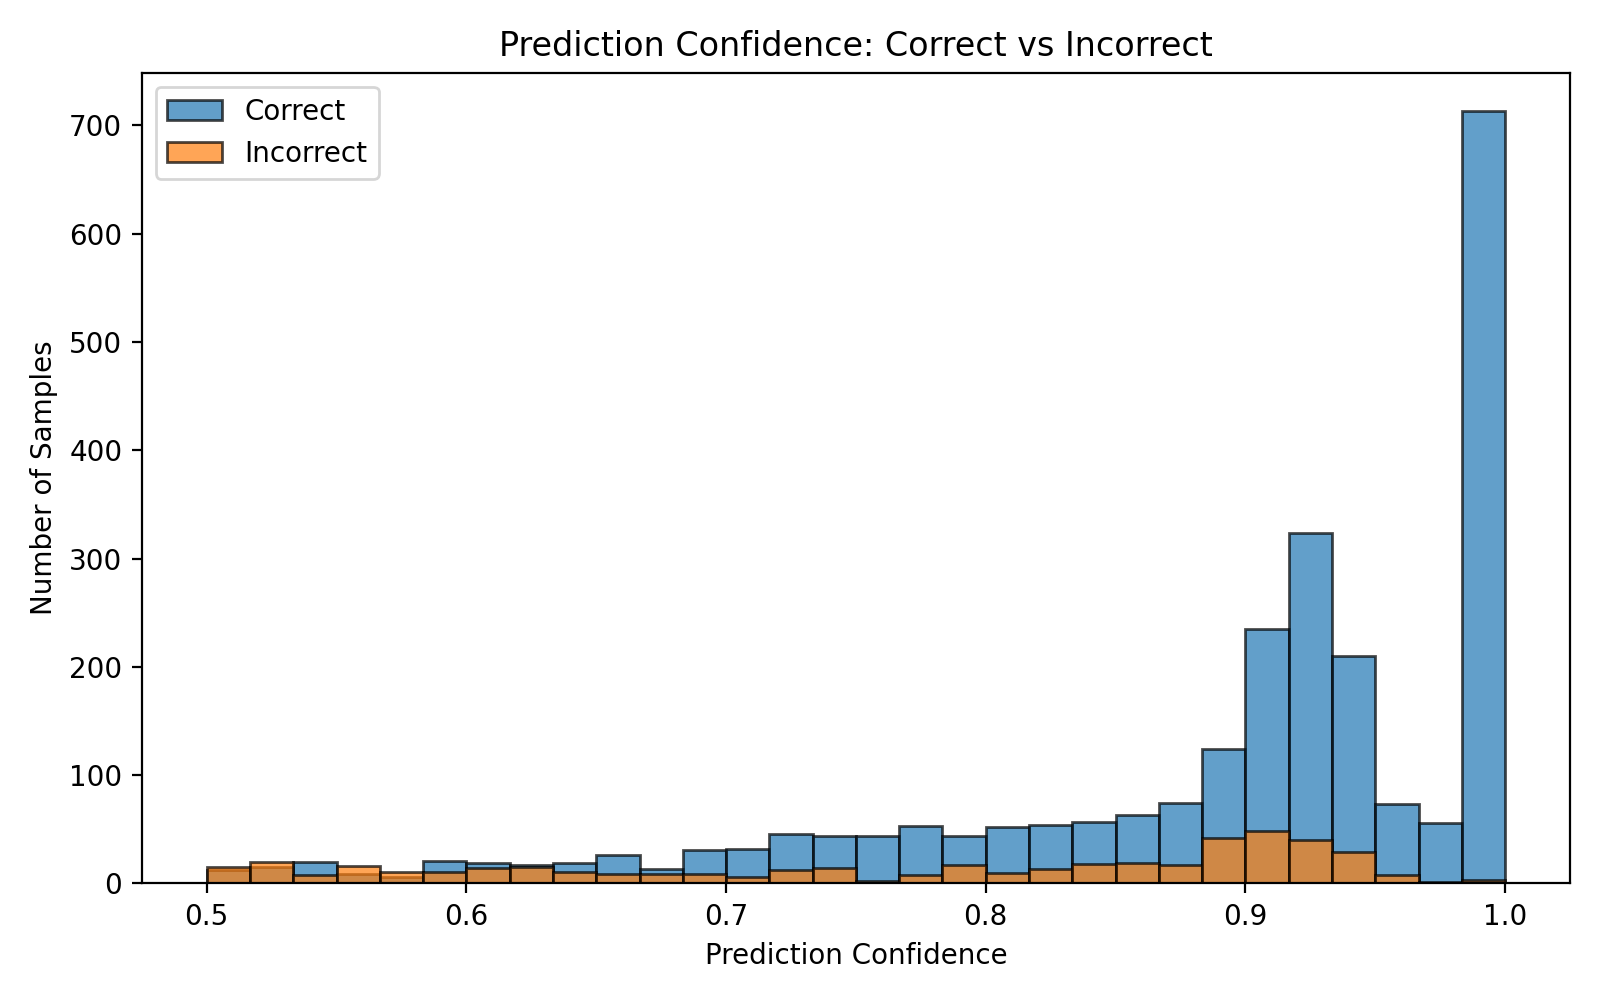
\includegraphics[width=0.5\linewidth]{figures/plots/confidence_correct_vs_incorrect.png}
    \caption{A histogram showing the spread of frequency of each confidence value the model returned. All correct classifications shown in \textbf{(Insert colour)} while incorrect classifications shown in \textbf{(Insert colour)}. An interesting bump in mistakes by the model is found in the \textbf{(What range? I think 0.8 to 0.9)}}
    \label{fig:conf_corr_vs_incorr_hist}
\end{figure}

Figure~\ref{fig:conf_corr_vs_incorr_hist} shows the distribution of all test instances by the models confidence in its classifications. A majority of classifications are correct with most falling with confidence of $0.8$ or greater. This makes sense when considering the metrics from Table~\ref{tab:metrics_table}. The focus in on the incorrect classifications as this gives info on the models mistakes. The incorrect bins sitting in the low range indicate typical errors in algorithms indicating where the model is unsure and likely guesses hoping to win the 50/50 chance. The focus is on the incorrect classifications with high confidence. Here the model was very sure of its decision but was incorrect which raises concerns as to why. 

One estimate is there is a correlation to the signal to noise ratio (SNR). In order to check this case we take the signal to noise ratio of each instance both from the \textit{Kepler} Archive and the simple equation using the transit depths. To analyse if this is the case, the false negatives which represent the misclassified eclipsing binaries need to be observed at different confidence ranges. As confidence can only sit between 0.5 (completely unsure) to 1.0 (extremely confident), the low range is set from $0.5$ to $0.7$, medium range from $0.7$ to $0.8$ and high for $0.8$ to $1.0$ \textbf{(Check these ranges for final publish}. 

\begin{figure}
    \centering
    \includegraphics[width=0.5\linewidth]{}
    \caption{Caption}
    \label{fig:placeholder}
\end{figure}
\section{Conclusion} \label{sec:Further_Steps}

This review has examined the transit photometry detection method and the challenges associated with its use. Various issues such as instrumental noise and stellar variability impact the ability for astronomers to detect potential exoplanets. To mitigate these difficulties, several space missions have been developed to monitor as many possible stars, using preprocessing steps to improve detectability.

\subsection{Further Steps}

Moving forward, machine learning is likely to play an increasingly important role in the field. Modern surveys have collected hundreds of thousands of light curves, making the analysis of all available data very impractical. With increasing dataset sizes and the continued challenge of false positives, convolutional neural networks (CNNs) provide a valuable addition to the research process. The challenges associated with transit detection and identification of astrophysical false positives remains central to the developing automated detection pipelines. As photometric surveys continue to expand in scale, CNNs can analyse large volumes of data with great efficiency and identify potential exoplanet candidates. Continued development of these techniques will be essential for improving the scientific return from current and future missions such as TESS and PLATO.

The \textit{Kepler} mission provides an extensive archive of high-precision stellar light curves, making it an ideal starting point for developing and testing machine learning approaches. Its large catalogue of classified signals offers a strong foundation for training and evaluating models before extending these techniques to TESS and PLATO.

\subsection{Proposed Project}

The question is whether a CNN can be trained to correctly classify light curves with minimal preprocessing in order to reduce computational cost and time. Current research often trains CNN models on cleaned and phase-folded light curves, where preprocessing makes the relevant transit features easier to identify. When managing hundreds of thousands of light curves, this preprocessing becomes highly time consuming. CNN pipelines are relatively straightforward to set up, reducing preprocessing time and allowing more time spent on analysis. However, this preprocessing is conducted to reduce the false positive rate leading to improved classification accuracy. The overall goal is to distinguish true planetary transits from common false positives and understand if speed can be gained without loss in quality.  

To apply this strategy of handling raw light curves, the first step is to establish a working CNN pipeline that runs without error. This begins with a simple case, making sure accuracy and other metrics can be calculated and plotted over time. To do this, a simple process such as uniform randomness is applied to introduce white noise to the data. The goal of this dataset is to represent cases of transits, eclipsing binaries, and normal stars. Using this synthetic data, the algorithm is trained to learn basic features of different light curve classes showing that the neural network is determining meaningful patterns through its feature maps. Once this model is developed, it works as a baseline for building into more complex algorithms. 

Real data is not nearly as clean and so this simple trained model will not be sufficient enough for handling realistic data. Once the first model works, the next step is the implementation of more realistic synthetic data. One effective way to do this is to overlay real stellar noise over the earlier synthetic data. This immediately makes the classification task more similar to real light curves, as the embedded features are now surrounded by realistic noise. This allows the CNN parameters to be adjusted to make is easier for the model to work with the data. 

This harder model must now look through the noise and detect the underlying pattern. Once this model is prepared, the next step is to move on to real data. \textit{Kepler} is the target domain for evaluating whether the earlier learning transfers. The \textit{Kepler} catalogue contains a large selection of confirmed and potential exoplanets, as well as eclipsing binaries to use in modelling. Using these, it is straightforward to build a model focused on the imperfections present in real light curves. Further adjustments can then be made to the training process to better analyse model performance and determine the most effective parameters for light curve classifications.

Overall, the training process is divided across three stages, creating a progressive approach. Each stage of learning is intended to prepare the CNN for the next. The final model is therefore expected to combine the basic feature learning of the first stage, the robustness of realistic variability and adaptation to real \textit{Kepler} data. This method allows the model to focus on one process at a time. Success is determined by whether this staged approach maintains strong classification performance throughout the training process. This would show that performance quality can be maintained while reducing preprocessing. 


\bibliographystyle{plain}
\bibliography{references}

\newpage 
\appendix \label{sec:Appendix}

\section{Transit Geometry} \label{sec:Transit_Geometry}

Several parameters describing the geometry of a transiting exoplanet system can be derived from the transit light curve. One of the most important is the impact parameter $(b)$, defined as the projected distance between the centre of the stellar disk and the transit chord:

\begin{align}
    b = \frac{a\cos{i}}{R_*}
\end{align}

Here, $a$ is the semi-major axis of the orbit, $i$ is the inclination, and $R_*$ is the radius of the star. These values are found using other methods but when combined give a good estimate for the impact parameter. Alongside the impact parameter, astronomers can get an accurate calculation of the transits duration as well. 

\begin{align}
    T = \frac{P}{\pi}\arcsin{\left(\frac{R_*}{a}\frac{\sqrt{(1-R_p/R_*)^2-b^2}}{\sin{i}}\right)}
\end{align}

$P$ is the period of the entire orbit which is easily resolved from the light curve and $R_p$ is the planets radius found using Equation~\ref{eq:flux_depth} \citep{2010exop.book...55W}. 

\section{Signal to Red Noise} \label{sec:Signal_to_Red_Noise}

\begin{align}
    S_{red}=\frac{\delta\sqrt{N_t}}{\sigma L^b}
\end{align}

$L$ is average number of data points in one transit and it is in a power law with b which quantifies covariance structure of the correlated noise. $\sigma$ is the weighted rms scatter of the unbinned data set. Lastly $\delta$ is the flux depth. \citep{2006MNRAS.373..799C} 

\section{Transit Detection Statistic} \label{sec:Transit_Detection_Statistic}

Many transit-search algorithms detect signals by comparing the average
stellar flux inside and outside a proposed transit window. In the
Box Least Squares (BLS) algorithm the transit depth can be expressed as

\begin{equation}
\delta = \overline{F}_{\mathrm{out}} - \overline{F}_{\mathrm{in}}
\end{equation}

where $\overline{F}_{\mathrm{in}}$ and $\overline{F}_{\mathrm{out}}$ denote
the mean flux during and outside the transit respectively. The statistical
significance of the detection can then be approximated by

\begin{equation}
S = \frac{\delta}{\sigma}\sqrt{N_{\mathrm{tr}}},
\end{equation}

where $\sigma$ is the photometric noise of the light curve and
$N_{\mathrm{tr}}$ is the number of observations within the transit window \citep{BLS_Algorithm}.

\section{Neural Network Metric Equations} \label{sec:NN_equations}

The following are the equations used to calculate the metrics used in this paper. T and F stand for True while P and N stand for Positive and Negative. R means Rate so for example FPR means False Positive Rate.
\begin{align}
    \text{Precision} = \frac{TP}{TP+FP}
\end{align}

\begin{equation}
    \text{Recall} = \frac{TP}{TP+FN}
\end{equation}

\begin{equation}
    \text{False Positive Rate} = 1 - \text{Recall}
\end{equation}

\begin{equation}
    F_1 = \frac{2TP}{2TP + FP + FN}
\end{equation}

\begin{align}
    AUC &= \int_0^1{\text{Recall}(FPR)d(FPR)}, \textbf{ where} \\
    FPR &= \frac{FP}{FP + TN}
\end{align}

\end{document}